%!TEX root = ../thesis-main.tex
%----------------------------------------------------------------------------------------
\chapter{Introduzione}
\label{chap:introduction}
%----------------------------------------------------------------------------------------

Il mondo del software ha scritto diverse decadi di storia. Sin dagli anni '50, quando i primi calcolatori programmabili hanno fatto il loro ingresso sul mercato, il software ha assunto un ruolo sempre più pervasivo nella vita quotidiana delle persone. Oltre ad essere parte integrante dei sistemi informativi delle aziende, lo possiamo trovare anche all'interno di automobili, elettrodomestici e tantissimi strumenti con la quale abbiamo a che fare nella nostra quotidianità. La crescente diffusione del software ha introdotto la necessità di progettare metodologie di sviluppo solide e versatili. Uno dei primi è il \textbf{modello a cascata} il quale struttura il processo di realizzazione del software in fasi sequenziali lineari. Il modello riprende la tipica organizzazione della produzione manifatturiera e fu progressivamente abbandonato con l'evolversi delle richieste del mercato. Successivamente prese piede il concetto di modelli iterativi come il \textbf{modello a spirale} in cui il processo di sviluppo è suddiviso in fasi multiple ripetute più volte (iterazioni). Gli ultimi decenni hanno dato vita a un nuovo modello, considerato lo standard dell'industria, la \textbf{metodologia agile}. Quest'ultima non rappresenta un unico modello, ma un insieme di modelli iterativi costruiti sulla base dei principi definiti all'interno del manifesto agile. Questi mettono in primo piano un ambiente autonomo e dinamico in cui sono fondamentali: cicli di sviluppo brevi, continui miglioramenti, la comunicazione col cliente e la consegna tempestiva di funzionalità. Il progetto esposto in questo documento introduce un evoluzione del concetto agile nato recentemente nel mondo dello sviluppo del software, conosciuto come ``DevOps".

\section{Contesto}

Con l'avvento di internet il concetto di software come un entità sviluppata e finita ha completamente cessato di esistere. Mediante la rete è diventato semplice ed efficiente distribuire un programma e fornire un ulteriore supporto attraverso aggiornamenti evolutivi e correttivi. Il fenomeno è cresciuto tanto da aver dato luce alla pratica del rilascio di applicazioni deliberatamente non complete, le quali attraverso il feedback degli utenti evolvono verso un prodotto finito. Il manifesto agile ha introdotto la cultura di emettere frequenti rilasci di nuove versioni del software, rendendo la distribuzione un punto cardine all'interno del ciclo di vita di esso. Dietro lo sviluppo rapido di nuove funzionalità è necessario il rilascio di queste altrettanto velocemente, la filosofia DevOps nasce per soddisfare questa esigenza.

\subsection{DevOps}
La metodologia DevOps (termine nato dalla contrazione di ``Development" ed ``Operations") si è formata intorno al 2008 con l'idea chiave di unire il team di sviluppo ed il team delle operazioni (infrastruttura). Spesso accade all'interno di organizzazioni di grandi dimensioni che questi due componenti fondamentali siano separati, ossia il rilascio dell'applicazione avviene dopo che il processo di sviluppo è terminato, senza la possibilità tra i due di coordinarsi durante l'esecuzione. La filosofia DevOps promuove l'unione dei due reparti per garantire la distribuzione di software di maggior qualità in modo continuo e controllato. Essi sono considerati un'unica entità e cooperano seguendo un modello come descritto nella figura \ref{fig:devops-process}.
\begin{figure}[htb]
	\centering
	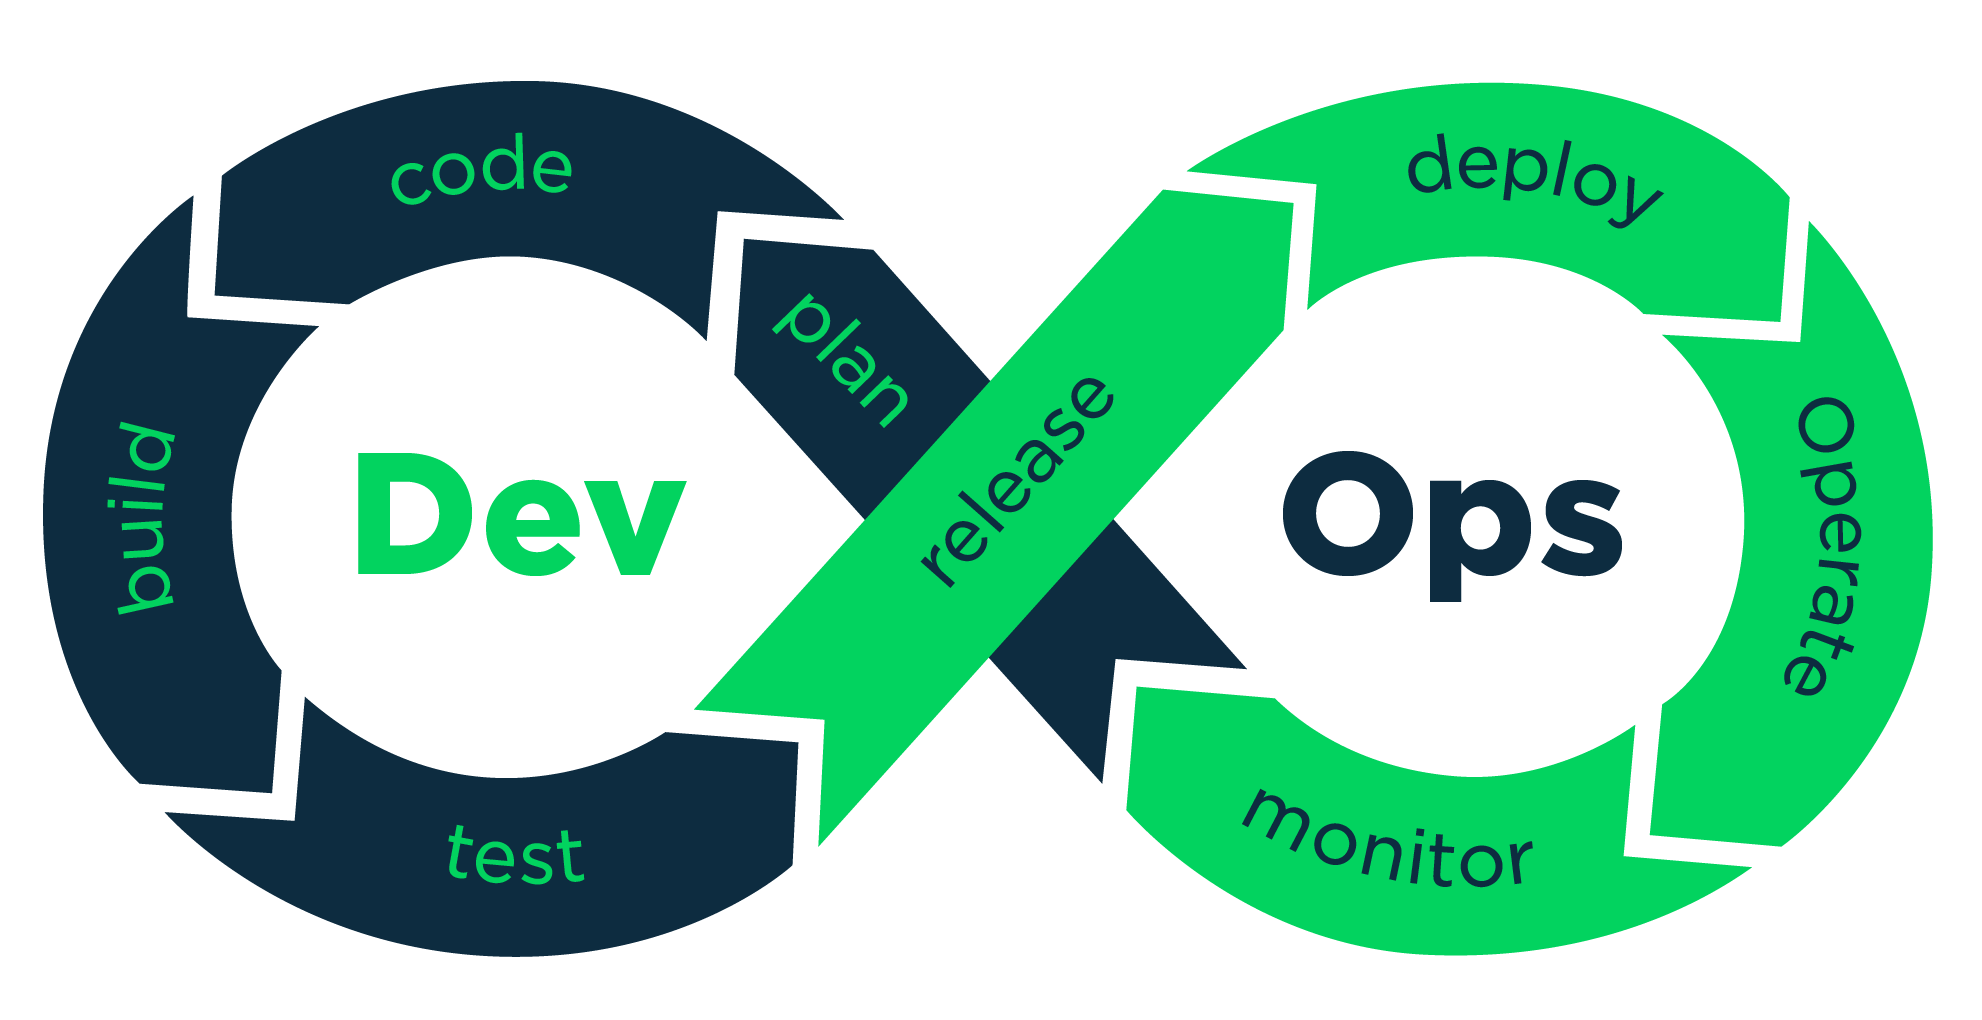
\includegraphics[width=.9\linewidth]{figures/devops-process.png}
	\caption{Le fasi della metodologia DevOps}
	\label{fig:devops-process}
	%https://italiancoders.it/introduzione-al-devops/
\end{figure}
Il modello mette in risalto le fasi e il rispettivo reparto di appartenenza, mentre le due fasi ``plan" e ``release" fungono da ponte per comporre un'unica entità.

Uno dei principi base della filosofia DevOps è l'utilizzo di pratiche di \ac{cicd}, ossia automazione dell'integrazione e distribuzione del software. Automatizzando le fasi descritte precedentemente si elimina l'intervento umano garantendo rilasci più rapidi e di maggior qualità.

\paragraph{Continuous integration} L'integrazione è costituita dalle operazioni di build e test del codice, essa diventa continuativa dal momento che si inserisce l'automazione nell'equazione. Un processo generalmente è formato secondo i seguenti step: (i) gli sviluppatori introducono nuovo codice nel progetto attraverso il software di \textit{version control} (per esempio git), (ii) un server ottiene la modifica ed esegue il build ed i test del progetto nella sua interezza, (iii) una volta completato il processo comunica l'esito delle operazioni agli sviluppatori. In questo modo le nuove parti di codice sono costantemente controllate riducendo al minimo la potenziale presenza di bug, migliorando in tutto e per tutto la qualità del progetto.
Un fattore molto importante è la stesura di test: più questi hanno una copertura maggiore, più saranno lenti nell'esecuzione e rallenteranno il processo di integrazione. È essenziale quindi calibrare la loro copertura secondo le esigenze del progetto, ricordando che una copertura totale migliora notevolmente la qualità del prodotto.

\paragraph{Continuous delivery} La distribuzione è l'insieme delle operazioni atte a consegnare il software agli utenti finali.

\paragraph{Le pipeline}

\subsection{Un software complesso: Alchemist}\label{sec:alchemist}

(Cos'è alchemist, utilizzo, tecnologie utilizzate, architettura, progettazione)

\paragraph{Open source}

\section{Obiettivi}

\subsection{Motivazioni}

\paragraph{Struttura della tesi}

La struttura di questo paper
